% !TEX root = ./../../_Thesis.tex

% section's Name and Label
\subsection{Visual Aberrations}
\label{subsec:VisualAberrations}

Visual aberrations are the main cause of visual impairment. Estimates indicate that there are about 153 million people with visual impairment due to uncorrected refractive errors \cite{Who2007}.
%
\citet{Thibos2002} defined standards for reporting of optical imperfections of eyes. The method of choice for assessing eye aberrations (\ie, describing its wavefront aberration) are the so called {\it Zernike polynomials}. They consist of a series of orthogonal polynomials over the area of a unitary circle (Figure~\ref{fig:unitcircle}) and can be expressed either in Cartesian $(X,Y)$ or polar  $(\theta, \rho)$ coordinate systems. The conversions between the two are given by: 

\begin{equation}
	\label{eq:pol2cart}
	\begin{alignat}{2}
		\rho &= \sqrt{x^2 + y^2}	& \theta &= \tan^{-1}(y/x)  \\
		   x &= \rho*\cos\theta	  &      y &= \rho*\sin\theta
	\end{alignat}
\end{equation}

%\noindent
%where $\rho = r/R$ is the normalized pupil radius.

\begin{figure}[!h]
	\centering
	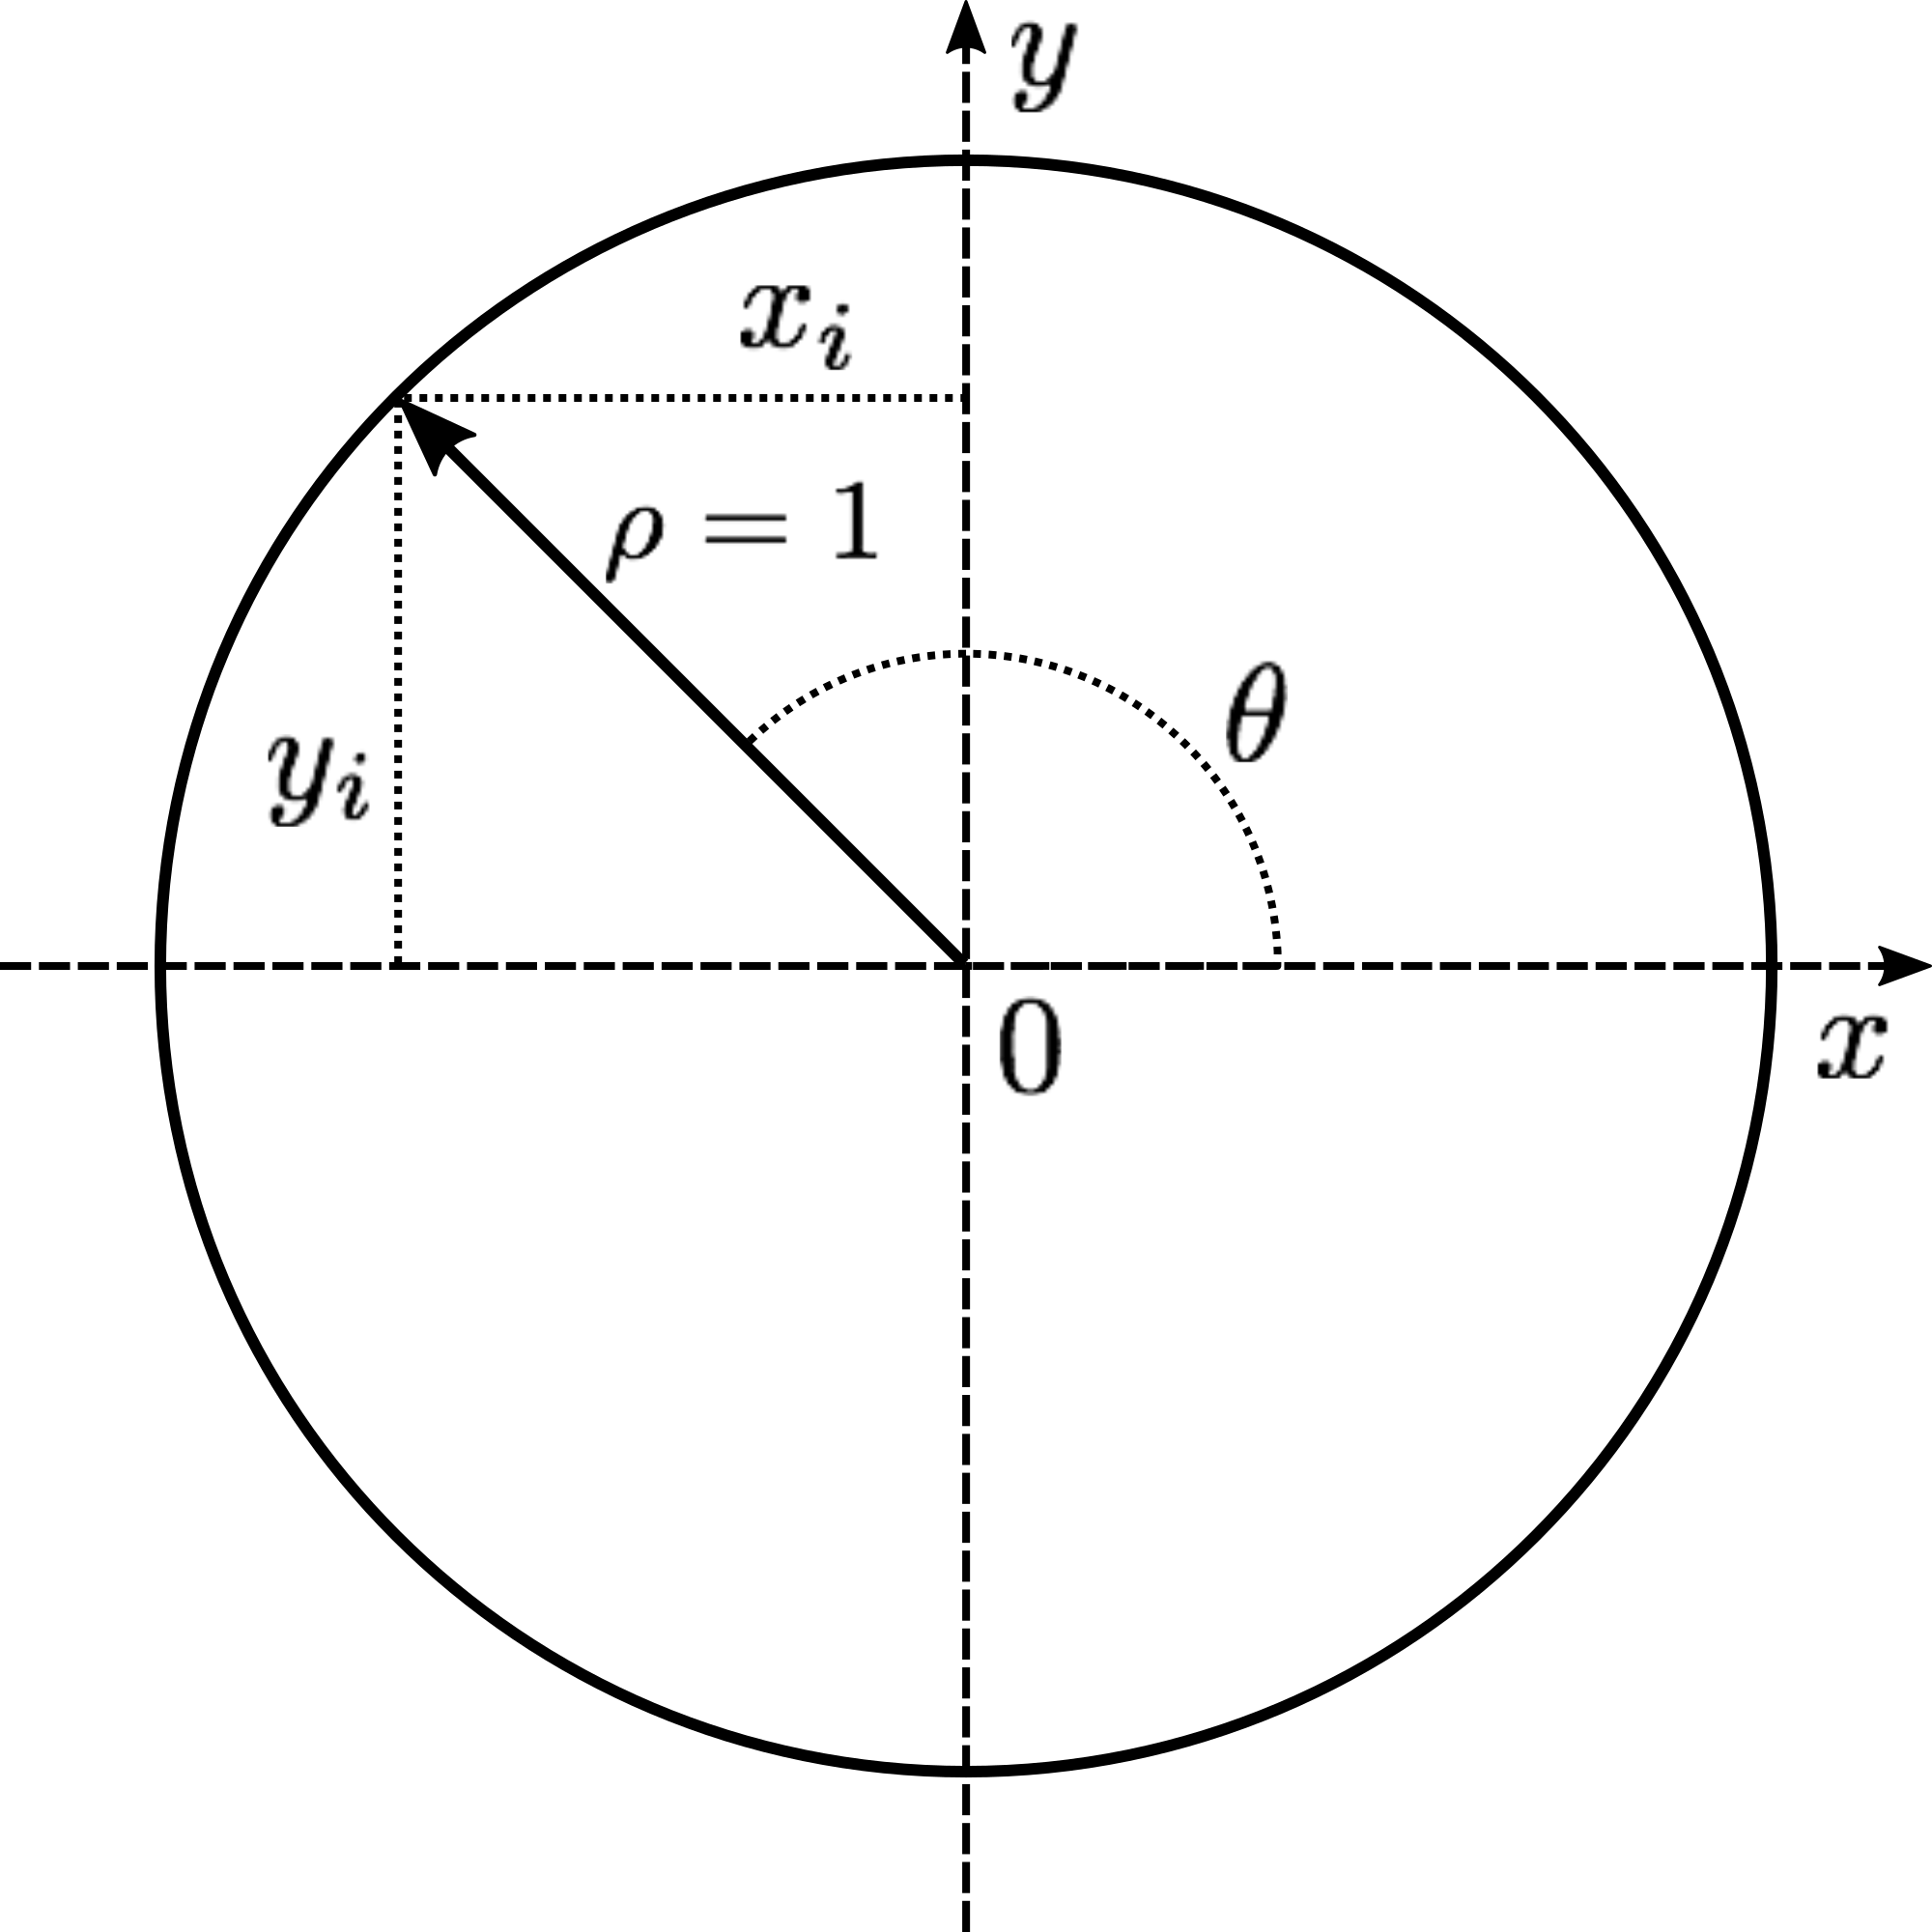
\includegraphics[width=0.45\linewidth]{__Images/02/unit_circle.png}
	\caption[The unit circle]{The unit circle.}
	\label{fig:unitcircle}
\end{figure}

There are several different normalization and numbering schemes for representing Zernike polynomials. Here we adopt a double indexing scheme ($Z^{m}_{n}$, where $n$ is the {\it order} and $m$ is the {\it frequency} -- see Figure~\ref{fig:zernike}).
% is useful for unambiguously describing these functions. 
Such a scheme is defined as:

\begin{equation}
	\label{eq:zernikedef}
	\[ Z^m_n(\rho,\theta) = 
		\begin{dcases*} 
			 N^m_n R^{|m|}_n (\rho)\cos m \theta, & for $m$ \geq 0,	\\ 
			-N^m_n R^{|m|}_n (\rho)\sin m \theta, & for $m$ < 0, 
		\end{dcases*} 
	\]
\end{equation}
where $N^m_n$, $R^{|m|}_n$ and the sinusoidal functions stand for the normalization factor, radial component, and azimuthal component, respectively. Such terms are fully described by \citet{Thibos2002}. Some of the {\it Zernike polynomials} (up to the $5^{th}$ order) are listed in Table~\ref{table:Zpoly} and illustrated in Figure~\ref{fig:zernike}. They can be applied directly to wavefront evaluation in the eye's pupil. In ophthalmology, the radial degree $n$ is the basis for classifying aberrations as lower-order ($n\leq2$) and higher-order ($n>2$). However, the vertical and horizontal tilt, as well the zeroth-order piston polynomial, are not considered in measurements of image focus quality \cite{Meister2010}.

%In Figure~\ref{fig:zernike}, it is possible to see some of those polynomials, which can be applied directly to wavefront evaluation in the eye's pupil. In ophthalmology, the radial degree $n$ is the basis for classifying aberrations as lower-order ($n\leq2$) and higher-order ($n>2$). 

\begin{table}[!b]
\centering
\caption{Zernike polynomials up to the fifth order.}
\label{table:Zpoly}
\begin{tabular}{cccll}
\hline
{\bf j} & {\bf n} & {\bf m} & {\bf Zernike Polynomials}	& {\bf Name}	\\ \hline

0	& 0	& 0		& $1$                            					& piston							\\
1	& 1	& -1	& $2\rho \sin\theta $								& vertical tilt						\\
2	& 1	& 1		& $2\rho \cos\theta $								& horizontal tilt					\\
3	& 2	& -2	& $\sqrt{6}\rho^2 \sin\theta$						& oblique astigmatism				\\
4	& 2	& 0		& $\sqrt{3}(2\rho^2-1)$								& defocus							\\
5	& 2	& 2		& $\sqrt{6}\rho^2 \cos\theta $						& vertical astigmatism				\\
6	& 3	& -3	& $\sqrt{8}\rho^3 \sin3\theta$ 						& vertical trefoil					\\
7	& 3	& -1	& $\sqrt{8}(3\rho^3-2\rho)\sin\theta$				& vertical coma						\\
8	& 3	& 1		& $\sqrt{8}(3\rho^3-2\rho)\cos\theta$				& horizontal coma					\\
9	& 3	& 3		& $\sqrt{8}\rho^3 \cos3\theta$						& oblique trefoil					\\
10	& 4	& -4	& $\sqrt{10}\rho^4 \sin4\theta$						& oblique quadrafoil				\\
11	& 4	& -2	& $\sqrt{10}(4\rho^4-3\rho^2)\sin2\theta$			& oblique secondary astigmatism		\\
12	& 4	& 0		& $\sqrt{5}(6\rho^4-6\rho^2+1)$						& primary spherical					\\
13	& 4	& 2		& $\sqrt{10}(4\rho^4-3\rho^2)\cos2\theta$			& vertical secondary astigmatism	\\
14	& 4	& 4		& $\sqrt{10}\rho^4 \cos4\theta$						& vertical quadrafoil				\\
15	& 5	& -5	& $\sqrt{12}\rho^5 \sin5\theta$						& vertical pentafoil				\\
16	& 5	& -3	& $\sqrt{12}(5\rho^5-4\rho^3)\sin3\theta$			& vertical secondary trefoil		\\
17	& 5	& -1	& $\sqrt{12}(10\rho^5-12\rho^3+3\rho)\sin\theta$	& vertical secondary coma			\\
18	& 5	& 1		& $\sqrt{12}(10\rho^5-12\rho^3+3\rho)\cos\theta$	& horizontal secondary coma			\\
19	& 5	& 3		& $\sqrt{12}(5\rho^5-4\rho^3)\cos3\theta$			& oblique secondary trefoil			\\
20	& 5	& 5		& $\sqrt{12}\rho^5 \cos5\theta$						& oblique pentafoil					\\ \hline
\end{tabular}
\end{table}


\begin{figure}[!t]
	\centering
	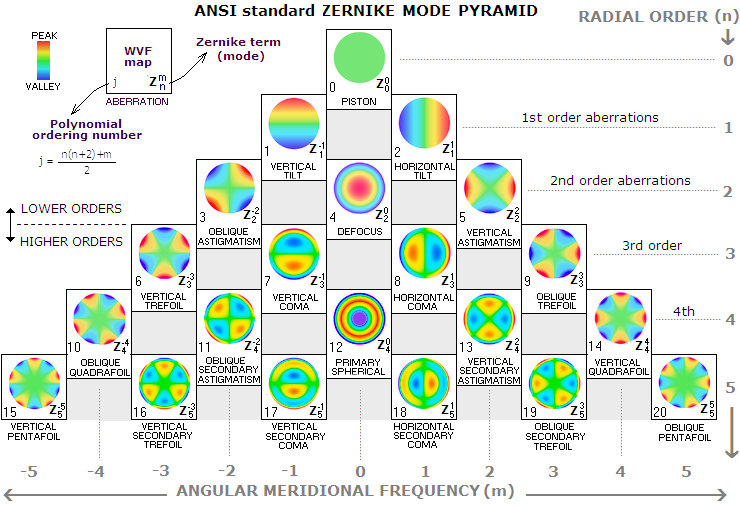
\includegraphics[width=0.98\linewidth]{__Images/02/zernike_pyramide.png}
	\caption[Zernike terms expansion pyramid]{The Zernike expansion pyramid: a function of term's radial degree (or order) $n$ and azimuthal frequency $m$ \cite{Sacek2015}.}
	\label{fig:zernike}
\end{figure}


%When the cornea has an irregularly shape or the eye's axial length is abnormal, light rays bends imperfectly, producing blurry vision. Figure ~\ref{fig:eye_diagram} shows a ray diagram for various eye visual aberrations. Myopic individuals have a natural advantage seeing up close, and objects are formed in front of the retina. Hyperopia causes the exact opposite of myopia and distant objects appear clear and close-up objects appear blurry. Under this condition, the image forms behind the retina. Astigmatism is a low-order aberration caused by a toric curvature in the cornea or crystallin.


